\documentclass[a4paper,11pt]{article}
\usepackage[utf8]{inputenc}
\usepackage[italian]{babel}
\usepackage[margin=1in]{geometry}
\usepackage{cite}
\usepackage{booktabs}
\usepackage{amsmath}
\usepackage{hyperref}
\usepackage{graphicx}

\title{Progetto di Sistema Closed-Loop BCI-Triggered con Guanto Soft-Robotico:\\
Linee Guida per la Neuroplasticità e la Riabilitazione\\
dell'Arto Superiore Post-Ictus}
\author{Studio di Fattibilità Ingegneristica e Clinica}
\date{\today}

\begin{document}

\maketitle

\begin{abstract}
Questo documento presenta una proposta metodologica e tecnologica per lo sviluppo di
un sistema riabilitativo closed-loop domiciliare destinato ai pazienti post-ictus.
Integrando la tecnologia Brain-Computer Interface (BCI) non invasiva basata su
elettroencefalografia (EEG) con un guanto soft-robotico pneumatico (SRG), il sistema
mira a promuovere la neuroplasticità Hebbiana attraverso la sincronizzazione temporale
tra l'intenzione motoria centrale e l'assistenza fisica periferica. L'architettura proposta
affronta i limiti storici della riabilitazione robotica passiva e della non-stazionarietà
dei segnali biologici tramite l'implementazione di un classificatore adattivo e di
algoritmi di controllo avanzati.
\end{abstract}

\newpage

% ---------------------------------------------------------------
\section{Framework Epidemiologico e Clinico (Il Bisogno)}
% ---------------------------------------------------------------
L'ictus cerebrale rappresenta una delle principali cause di disabilità neurologica
a lungo termine a livello globale. Come evidenziato dai dati epidemiologici della
World Stroke Organization \cite{feigin2025world}, l'impatto sociosanitario di questa
patologia è in costante crescita: oltre 93 milioni di casi prevalenti, circa
160 milioni di anni di vita persi a causa della disabilità (DALYs) e un costo economico
globale stimato superiore a 890 miliardi di dollari USA.

Tra il 55\% e il 75\% dei sopravvissuti presenta un deficit motorio cronico
dell'arto superiore che compromette l'autonomia nelle attività quotidiane (ADL)
\cite{proietti2024combining}. Donkor \cite{donkor2018stroke} contestualizza questa
cifra nella prospettiva della qualità della vita: l'ictus è la seconda causa di morte
al mondo e causa disabilità permanente grave in circa la metà dei sopravvissuti,
con elevato impatto su autonomia, vita lavorativa e carico assistenziale sui familiari.
Questa combinazione di alta prevalenza e alta disabilità residua giustifica la ricerca
di soluzioni tecnologiche avanzate che possano erogare terapia a domicilio con
un'intensità paragonabile a quella dei reparti di riabilitazione specialistica.

La ricerca clinica recente indica che l'efficacia dei trattamenti riabilitativi
tradizionali è fortemente limitata da un deficit di dosaggio terapeutico.
L'analisi sistematica condotta da Newton et al.\ \cite{newton2023dose} evidenzia
come il tempo effettivo dedicato all'esercizio terapeutico attivo (\textit{time on task})
all'interno delle sessioni convenzionali oscilli mediamente tra gli 8 e i 44 minuti
al giorno — ampiamente inferiore alle dosi raccomandate per indurre riorganizzazione
corticale stabile. Un paradosso clinico emerge: i pazienti con compromissione più
severa ricevono dosi di terapia attiva significativamente inferiori proprio per
l'elevato sforzo richiesto senza strumenti di assistenza modulabili.

% ---------------------------------------------------------------
\section{Il Limite Neurofisiologico e la Plasticità Hebbiana}
% ---------------------------------------------------------------
I trattamenti riabilitativi puramente passivi mostrano un'efficacia limitata nel
promuovere il recupero funzionale a lungo termine. La spiegazione risiede nei
meccanismi neurobiologici della plasticità sinaptica attività-dipendente.

La riorganizzazione delle mappe corticali dipende dal principio della plasticità
Hebbiana o \textit{Spike-Timing-Dependent Plasticity} (STDP). Come dimostrato da
Biasiucci et al.\ \cite{biasiucci2018brain} e Krueger et al.\ \cite{krueger2024hebbian},
l'induzione di modificazioni sinaptiche stabili richiede la coincidenza temporale
(entro circa 300 ms) tra l'attivazione della corteccia motoria associata all'intenzione
di movimento (segnale pre-sinaptico) e il feedback visuo-propriocettivo afferente
generato dal movimento dell'arto (segnale post-sinaptico).

Nelle bande di frequenza $\mu$ (8--12 Hz) e $\beta$ (13--30 Hz), l'immaginazione
del movimento (\textit{Motor Imagery}, MI) si manifesta come desincronizzazione
correlata all'evento (ERD) localizzata sulle aree motorie controlaterali (C3/C4).
Quando il sistema BCI rileva questa ERD e la usa come trigger istantaneo per
attivare l'ortesi, si realizza la contingenza temporale necessaria. Al contrario,
un'attivazione casuale (protocollo Sham) non produce incrementi significativi
della coerenza corticomuscolare (CMC) in banda $\beta$ \cite{krueger2024hebbian}
né miglioramenti clinici rilevanti \cite{kim2025efficacy}.

Il biomarcatore di questa riorganizzazione è misurabile in tempo reale:
Rustamov et al.\ \cite{rustamov2025ipsihand} dimostrano che il theta-gamma
cross-frequency coupling (CFC) sugli elettrodi C3/C4 aumenta proporzionalmente
al recupero motorio nel corso delle sessioni BCI — correlazione positiva
significativa che conferma il CFC come proxy neurobiologico dell'efficacia
del trattamento.

% ---------------------------------------------------------------
\section{Il Limite dell'Hardware Passivo}
% ---------------------------------------------------------------
Le ortesi motorie tradizionali e i guanti robotici commerciali privi di accoppiamento
intenzionale presentano un limite intrinseco. Lo studio di Wang et al.\
\cite{wang2023effectiveness} ha confrontato un guanto soft-robotico passivo con
la stimolazione magnetica transcranica ripetitiva (rTMS). I risultati mostrano che,
sebbene il guanto migliori la Fugl-Meyer Assessment (FMA-UE) facilitando la
mobilitazione articolare, esso non produce variazioni significative nella soglia
motoria a riposo (\textit{Resting Motor Threshold}, RMT) né nell'ampiezza dei
potenziali evocati motori (MEP). L'intervento centrale (rTMS) agisce invece
direttamente sull'eccitabilità sinaptica corticale.

Questo limite evidenzia la necessità di integrare hardware periferico con rilevamento
centrale. Un guanto soft-robotico BCI-triggered unisce i benefici della mobilizzazione
meccanica (prevenzione di contratture, stimolazione dei propriocettori muscolari
\cite{osuagwu2020home}) con la modulazione attiva dei circuiti corticali, trasformando
l'ortesi da strumento passivo a facilitatore di neuroplasticità.

% ---------------------------------------------------------------
\section{Validazione Neuro-Clinica e Precedenti Regolatori}
% ---------------------------------------------------------------
L'efficacia della terapia riabilitativa basata su BCI-ortesi è supportata da un
solido corpo di prove cliniche e neurofisiologiche:

\begin{itemize}
    \item \textbf{Efficacia Clinica Quantificabile (Meta-analisi):}
    La meta-analisi di Ren et al.\ \cite{ren2024effect}, che analizza 10 RCT
    per 290 pazienti totali, conferma l'efficacia del trattamento BCI-FES/BCI-robot
    rispetto alla terapia convenzionale (SMD\,=\,0.50, 95\% CI: 0.26--0.73).

    \item \textbf{Efficacia Clinica Quantificabile (Trial Prospettico):}
    Premchand et al.\ \cite{premchand2025personalized} riportano, in un trial
    clinico prospettico su 4 pazienti cronici con sistema multimodale EEG+fNIRS
    e guanto soft-robotico, guadagni medi di FMA\,=\,$8.75 \pm 1.84$ e
    ARAT\,=\,$5.25 \pm 2.17$ a settimana 12 rispetto al baseline — superiori
    a tutti i trial BCI-SR precedenti confrontati retrospettivamente.

    \item \textbf{Modificazioni della Connettività Corticale:}
    Gli studi fMRI di Ma et al.\ \cite{ma2024motor} dimostrano che il recupero
    guidato da MI-BCI è associato a cambiamenti plastici oggettivi: incremento
    dell'attività spontanea a bassa frequenza (zALFF) e della coerenza regionale
    (ReHo) nell'area sensomotoria primaria dell'emisfero leso
    ($r = 0.425$, $P < 0.05$).

    \item \textbf{Evidenza su Pazienti Cronici Gravi:}
    Rustamov et al.\ \cite{rustamov2025ipsihand}, in un trial prospettico su
    30 pazienti cronici emiparetici (12 settimane, sistema IpsiHand), riportano
    miglioramenti significativi sia prossimali che distali dell'arto superiore,
    indipendenti dalla somministrazione di Botox. Il theta-gamma CFC è aumentato
    bilateralmente sugli elettrodi motori C3/C4 con correlazione positiva al
    recupero motorio.

    \item \textbf{Precedente Regolatorio (FDA):}
    Il sistema IpsiHand (Neurolutions) \cite{rustamov2025ipsihand} è il primo
    BCI per riabilitazione motoria post-ictus ad ottenere autorizzazione FDA di
    Classe II, dimostrando la fattibilità commerciale e clinica di sistemi
    domiciliari BCI-ortesi. Questo costituisce il \textit{predicate device}
    diretto per la nostra classificazione regolamentare.
\end{itemize}

% ---------------------------------------------------------------
\section{Architettura del Sistema Proposto}
% ---------------------------------------------------------------
La soluzione ingegneristica integra tre moduli principali, affrontando usabilità
domestica, variabilità del segnale EEG e personalizzazione del trattamento.

\begin{figure}[h]
\centering
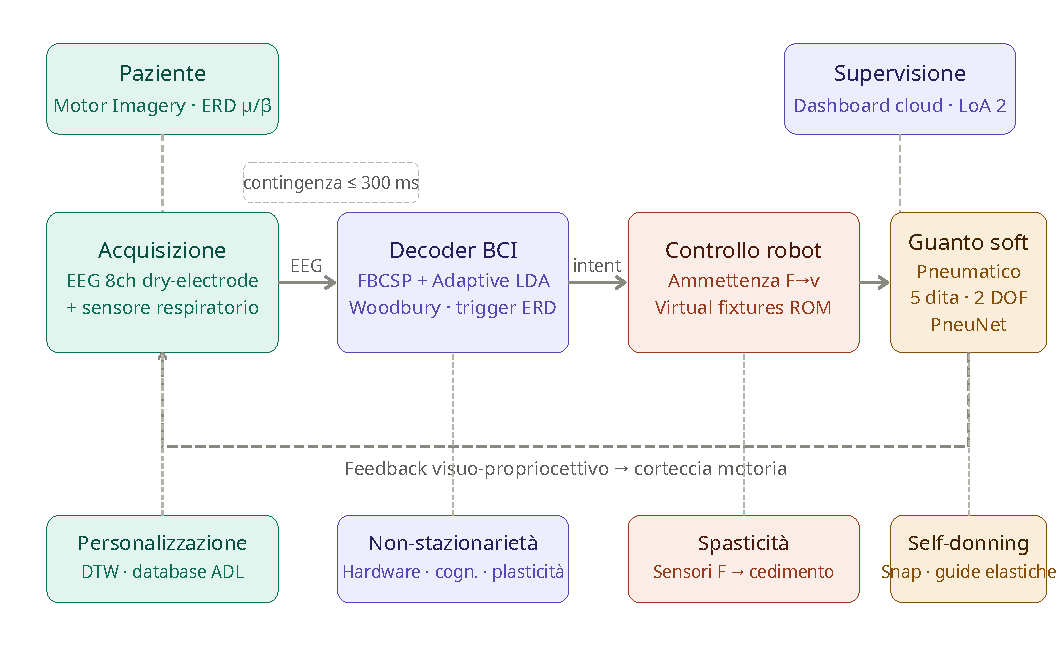
\includegraphics[width=\textwidth]{bci_glove_system_diagram_v2.pdf}
\caption{Architettura closed-loop del sistema BCI-triggered soft robotic glove.
Il loop feedforward (sinistra$\to$destra) mostra la catena paziente $\to$
acquisizione EEG+sensore respiratorio $\to$ decoder FBCSP+LDA adattivo $\to$
controllo robot (virtual fixtures + ammettenza) $\to$ guanto soft pneumatico.
La freccia tratteggiata chiude il loop con il feedback visuo-propriocettivo.
Il riquadro superiore indica la supervisione remota del terapista via dashboard.
La latenza complessiva target è $\leq$300\,ms per garantire la contingenza Hebbiana.}
\label{fig:architettura}
\end{figure}

\subsection{Perché robot e non BCI-FES}

Perché un guanto robotico e non la stimolazione elettrica funzionale (FES)?
La FES BCI-triggered è la principale alternativa tecnologica e produce anch'essa plasticità Hebbiana \cite{biasiucci2018brain}. 
Il motivo per cui non è la soluzione corretta in questo contesto specifico — il domicilio non supervisionato — è di natura pratica, 
non teorica. Il posizionamento degli elettrodi FES sull'avambraccio richiede identificazione precisa dei punti motori, che varia tra 
sessioni e richiede verifica da personale qualificato. Un paziente emiparético non può eseguire questo setup autonomamente con una sola mano. 
Il guanto soft self-donning \cite{proietti2024combining} risolve esattamente questo problema: non ci sono parametri di posizionamento 
da ottimizzare, il feedback meccanico è deterministico indipendentemente dalla sessione, e il design monomanuale è stato validato su 
pazienti con funzione residua dell'arto superiore di grado moderato-severo. La scelta del guanto non è quindi una preferenza tecnologica — 
è un vincolo imposto dal setting domiciliare non supervisionato che costituisce il bisogno clinico definito in apertura.


\subsection{Modulo Hardware e Usabilità Domestica}
Il dispositivo periferico è basato sull'architettura soft-robotica di Proietti et al.\
\cite{proietti2024combining}: guanto in materiale tessile leggero con attuatori
pneumatici PneuNet in elastomero termoplastico integrati sul dorso delle dita.
Per consentire l'uso monomanuale indipendente a domicilio da parte di pazienti
emiparetici, il guanto incorpora snap colorati, guide elastiche e design
\textit{self-donning} \cite{proietti2024combining, fiska2025integration}.

\paragraph{Perché è fattibile adesso e non 5 anni fa.}
Tre convergenze tecnologiche recenti rendono questo sistema deployabile nel 2025:
(1) Gli elettrodi dry-electrode (no-gel) di qualità clinica per EEG sono disponibili
commercialmente a costo ridotto dal 2021+, eliminando la necessità di personale per
la preparazione del scalpo.
(2) Il riconoscimento dell'intento motorio tramite FBCSP gira in tempo reale su
hardware edge (es.\ Raspberry Pi 4) con latenza documentata $<$50\,ms \cite{wu2024adaptive}.
(3) Gli attuatori soft pneumatici in silicone colato sono producibili con costi di
materiale $<$50€ per guanto tramite stampa 3D di stampi, abbassando la barriera di
prototipazione da centinaia di migliaia a poche migliaia di euro.

\subsection{Classificazione Adattiva dei Segnali EEG}
La non-stazionarietà del segnale EEG ha tre cause documentate \cite{wu2024adaptive}:
(a) variazioni hardware (deriva dell'impedenza degli elettrodi a secco);
(b) fluttuazioni degli stati cognitivi del paziente (attenzione, vigilanza, motivazione);
(c) cambiamenti neurali indotti dalla plasticità a breve termine dovuta alla pratica
del task stesso. La terza causa è paradossalmente un segnale di efficacia: il segnale
cambia perché il paziente sta migliorando. Per tutte e tre, il sistema implementa un
classificatore adattivo LDA \cite{wu2024adaptive} che aggiorna ricorsivamente i
parametri ad ogni coppia di trial validi:
\begin{equation}
\mu_i(t) = (1 - UC_{\mu})\,\mu_i(t-1) + UC_{\mu}\,x_i(t)
\end{equation}
La matrice di covarianza inversa $\Sigma(t)^{-1}$ viene aggiornata tramite l'identità
di Woodbury, garantendo stabilità del feedback visuo-motorio in tempo reale.

\subsection{Personalizzazione basata sui Dati e Sincronizzazione Respiratoria}
Il sistema applica il principio della riabilitazione personalizzata di Premchand et al.\
\cite{premchand2025personalized}: la cinematica articolare del paziente viene mappata
e confrontata, tramite Dynamic Time Warping (DTW), con un database di movimenti
normativi. Vengono così identificate le specifiche ADL in cui il paziente mostra
deficit significativi (es.\ presa cilindrica o presa a pinza), evitando task irrilevanti
per il suo profilo di menomazione.

La comparsa del cue visivo di Motor Imagery viene sincronizzata con la fase inspiratoria
del ciclo respiratorio tramite un sensore addominale \cite{premchand2025personalized}.
Questa sincronizzazione riduce la dispersione basale del segnale di ossigenazione (HbO)
e stabilizza la baseline EEG, aumentando l'accuratezza di decodifica della BCI.

\subsection{Integrazione dei Concetti di Robotica e Controllo}
\begin{itemize}
    \item \textbf{LoA 2 — Shared Control:} Il paziente esercita il controllo di
    alto livello (\textit{intent planner}) tramite la BCI; il controllore del guanto
    gestisce in autonomia l'esecuzione della traiettoria fisica e la sicurezza
    biomeccanica.
    \item \textbf{Admittance Control ($F \to v$):} Sensori piezoelettrici flessibili
    rilevano le forze di reazione dell'utente; il controllore adatta pressione e
    velocità degli attuatori al tono muscolare del paziente, prevenendo forzature
    articolari in presenza di spasticità.
    \item \textbf{Virtual Fixtures:} Vincoli geometrici software impediscono
    all'ortesi di superare il ROM di sicurezza configurato dal terapista per
    ciascuna articolazione del paziente.
    \item \textbf{Teleoperazione Asincrona:} Il terapista supervisiona da remoto
    via dashboard cloud, definendo soglie di confidenza della BCI e target di
    esercizio. Il loop di controllo locale in tempo reale garantisce sicurezza
    indipendentemente dalla latenza di rete.
\end{itemize}

\newpage
% ---------------------------------------------------------------
\section{Analisi delle Criticità e Mitigazioni}
% ---------------------------------------------------------------
\begin{table}[h]
\centering
\label{tab:criticita}
\begin{tabular}{@{}p{6cm}p{7.5cm}@{}}
\toprule
\textbf{Criticità Rilevata} & \textbf{Strategia di Mitigazione} \\ \midrule
Non-stazionarietà del segnale EEG
  & Adaptive LDA con ricalcolo ricorsivo (Woodbury); la deriva da plasticità a
    breve termine è riclassificata come segnale di efficacia \cite{wu2024adaptive}. \\[4pt]
Instabilità del feedback BCI
  & Integrazione temporale dei segnali (\textit{leaky integrator}) per ridurre
    falsi positivi da artefatti muscolari transitori. \\[4pt]
Ipertono muscolare e spasticità
  & Controllo in ammettenza: il guanto cede proporzionalmente alla resistenza
    involontaria del paziente. \\[4pt]
Rischio di lesioni articolari
  & Virtual Fixtures software sui limiti ROM configurabili per paziente. \\[4pt]
Basso coinvolgimento / abbandono
  & Task personalizzati su ADL reali e significativi per il paziente
    \cite{premchand2025personalized}; gamification del semaforo BCI. \\[4pt]
Complessità di calibrazione
  & Sincronizzazione respiratoria per stabilizzazione baseline; calibrazione
    assistita automaticamente dalla prima sessione \cite{premchand2025personalized}. \\[4pt]
Difficoltà di indossamento monomanuale
  & Design self-donning con snap colorati e guanto di supporto
    \cite{proietti2024combining}. \\[4pt]
Variabilità inter-paziente
  & La meta-analisi Ren et al.\ \cite{ren2024effect} identifica questo come
    fattore confondente primario (SMD CI largo); mitigato dalla personalizzazione
    DTW del sistema \cite{premchand2025personalized}. \\ \bottomrule
\end{tabular}
\caption{Matrice delle Criticità e Strategie di Mitigazione}
\end{table}

% ---------------------------------------------------------------
\section{Quadro Regolatorio e Modello di Business}
% ---------------------------------------------------------------

\subsection{Classificazione Regolatoria}

\paragraph{Stati Uniti (FDA).}
Il dispositivo rientra nella \textbf{Classe II FDA} con percorso di clearance
\textbf{510(k)}. Il \textit{predicate device} diretto è il sistema IpsiHand
(Neurolutions), primo BCI per riabilitazione motoria post-ictus ad ottenere
autorizzazione FDA de Novo — stesso paradigma EEG-triggered exoskeleton,
stessa classificazione di rischio \cite{rustamov2025ipsihand}.

\paragraph{Unione Europea (EU MDR 2017/745).}
In Europa il dispositivo è classificato \textbf{Classe IIb} secondo il
Regolamento EU 2017/745, Allegato VIII, Regola 10. La Regola 10 si applica
ai dispositivi terapeutici attivi che somministrano o scambiano energia con
il paziente: il guanto pneumatico BCI-triggered è un dispositivo attivo
terapeutico non invasivo a rischio medio-alto, che non rientra né nella
Classe I (nessuna interazione energetica con il corpo) né nella Classe III
(non impiantabile, non a contatto con il sistema nervoso centrale).

La \textbf{differenza pratica} rispetto al percorso FDA è rilevante:
la Classe IIb EU richiede il coinvolgimento di un \textit{Notified Body}
accreditato per la valutazione della conformità tecnica e clinica, la
redazione di un \textit{Clinical Evaluation Report} completo e la
registrazione su EUDAMED. Il termine di compliance per i dispositivi
Classe IIb non impiantabili è il 31 dicembre 2028, con periodo di transizione
dalla precedente Direttiva MDD.

\subsection{Evidenza clinica richiesta per la submission}
Il precedente IpsiHand definisce anche la dimensione del trial attesa dalla 
FDA per una submission 510(k) in questa indicazione: 30 pazienti cronici, 12 settimane di trattamento, endpoint primario 
FMA-UE con MCID di 5--6 punti \cite{rustamov2025ipsihand}. La meta-analisi di Ren et al.\ \cite{ren2024effect} conferma che 
questo endpoint è accettato dalla letteratura peer-reviewed come misura di efficacia clinicamente significativa 
(SMD,=,0.50, 95 \% CI: 0.26--0.73 su 290 pazienti aggregati). 
Per il percorso EU MDR Classe IIb, il Clinical Evaluation Report dovrà dimostrare equivalenza clinica con IpsiHand — 
stesso paradigma EEG-triggered ortesi, stesso endpoint — o condurre un trial pivotal di dimensione analoga con controllo attivo. 
Questo non è un ostacolo imprevedibile: è un percorso con precedente diretto e costo stimabile.


\subsection{Identificazione del Payer e Modello di Rimborso}
La sostenibilità economica del sistema si basa su tre canali:

\begin{enumerate}
    \item \textbf{Payer primario — SSN / NHS europeo (rimborso di episodio):}
    Il sistema si posiziona come sostituzione della fisioterapia
    convenzionale post-acuta per l'arto superiore. In molti sistemi sanitari
    europei la riabilitazione post-stroke è rimborsata come \textit{line item}
    esistente (DRG, prestazioni ambulatoriali o ADI). Il dispositivo non crea
    una nuova voce di rimborso: sostituisce le sessioni di fisioterapia
    convenzionale con sessioni domiciliari BCI-robotiche supervisionate
    da remoto, riducendo il costo per sessione (assenza di trasporto,
    valorizzazione del tempo del terapista su più pazienti in parallelo).

    \item \textbf{Payer secondario — Assicurazioni sanitarie integrative:}
    La teleriabilitazione è documentata come cost-effective rispetto alla
    terapia in-clinic per la riabilitazione post-stroke, con rapporti
    costo-utilità favorevoli in multipli sistemi sanitari. I piani assicurativi
    integrativi in Italia, Germania e Francia stanno progressivamente
    includendo la teleriabilitazione nei pacchetti di copertura, creando
    un secondo canale di rimborso.

    \item \textbf{Modello SaaS per il terapista:}
    Il hardware viene venduto o noleggiato al paziente (o al reparto di
    neuroriabilitazione); la piattaforma di supervisione remota, il
    dashboard clinico e gli aggiornamenti del modello BCI sono erogati come
    servizio in abbonamento mensile fatturato al reparto, analogamente ai
    modelli già adottati da aziende di telerehab nel settore MSK.
\end{enumerate}

% ---------------------------------------------------------------
\section{Piano di Sviluppo e Prototipazione (1 Mese)}
% ---------------------------------------------------------------
Per convalidare la fattibilità dell'architettura, viene pianificato un piano
di sviluppo rapido della durata di un mese per un prototipo funzionale a tre dita:

\begin{enumerate}
    \item \textbf{Settimana 1 — Classificatore Off-line}
    \begin{itemize}
        \item Acquisizione dataset EEG pubblici (BCI Competition IV, dataset 2a)
        con registrazioni di Motor Imagery dell'arto superiore.
        \item Implementazione Python di FBCSP e Adaptive LDA \cite{wu2024adaptive}.
        \item Validazione della classificazione simulando non-stazionarietà del segnale.
    \end{itemize}
    \item \textbf{Settimana 2 — Hardware Guanto Pneumatico}
    \begin{itemize}
        \item Ortesi semplificata a tre dita (pollice, indice, medio) con attuatori
        in silicone colato in stampi 3D.
        \item Integrazione sensori di flessione resistivi e sensori piezoelettrici.
        \item Unità di controllo pneumatica: elettrovalvole a solenoide + mini-pompa
        12V su microcontroller Arduino.
    \end{itemize}
    \item \textbf{Settimana 3 — Integrazione Software e Controllo}
    \begin{itemize}
        \item Codice di controllo su microcontroller per attuazione pneumatica.
        \item Loop di controllo in ammettenza basato sui sensori di pressione.
        \item Funzioni di sicurezza: interruzione immediata al superamento delle soglie
        geometriche (virtual fixtures).
    \end{itemize}
    \item \textbf{Settimana 4 — Validazione Closed-Loop}
    \begin{itemize}
        \item Connessione via Bluetooth tra elaborazione EEG (Python) e controllo
        guanto (microcontroller).
        \item Test end-to-end su utente sano: MI $\to$ ERD rilevata $\to$
        trigger guanto $\to$ estensione/flessione assistita.
        \item Misura latenza complessiva (target: $\leq$300 ms per contingenza
        Hebbiana \cite{biasiucci2018brain, krueger2024hebbian}) e stesura
        report tecnico finale.
    \end{itemize}
\end{enumerate}

\newpage
\bibliographystyle{unsrt}
\begin{thebibliography}{10}

\bibitem{feigin2025world}
Valery~L. Feigin, Michael Brainin, Bo~Norrving, Sheila~O. Martins, Jeyaraj
  Pandian, Patrice Lindsay, Maria~F. Grupper, and Ilari Rautalin.
\newblock World stroke organization: Global stroke fact sheet 2025.
\newblock {\em International Journal of Stroke}, 20(2):132--144, 2025.

\bibitem{donkor2018stroke}
Emmanuel~S. Donkor.
\newblock Stroke in the 21st century: A snapshot of the burden, epidemiology,
  and quality of life.
\newblock {\em Stroke Research and Treatment}, 2018:3238165, 2018.

\bibitem{newton2023dose}
Sarah~P. Newton, Emily~J. Dalton, Jia~Y. Ang, Marlena Klaic, Vincent Thijs,
  and Kathryn~S. Hayward.
\newblock Dose, content, and context of usual care in stroke upper limb motor
  interventions: A systematic review.
\newblock {\em Clinical Rehabilitation}, 37(11):1437--1450, 2023.

\bibitem{biasiucci2018brain}
A.~Biasiucci, R.~Leeb, I.~Iturrate, S.~Perdikis, A.~Al-Khodairy, T.~Corbet,
  A.~Schnider, T.~Schmidlin, H.~Zhang, M.~Bassolino, D.~Viceic, P.~Vuadens,
  A.~G. Guggisberg, and J.~d. R.~Mill{\'a}n.
\newblock Brain-actuated functional electrical stimulation elicits lasting arm
  motor recovery after stroke.
\newblock {\em Nature Communications}, 9:2421, 2018.

\bibitem{krueger2024hebbian}
Johanna Krueger, Richard Krauth, Christoph Reichert, Serafeim Perdikis, Susanne
  Vogt, Tessa Huchtemann, Stefan D{\"u}rschmid, Almut Sickert, Juliane
  Lamprecht, Almir Huremovic, Michael G{\"o}rtler, Slawomir~J. Nasuto,
  I.-Chin Tsai, Robert~T. Knight, Hermann Hinrichs, Hans-Jochen Heinze, Sabine
  Lindquist, Michael Sailer, Jose~del R.~Mill{\'a}n, and Catherine~M.
  Sweeney-Reed.
\newblock Hebbian plasticity induced by temporally coincident bci enhances
  post-stroke motor recovery.
\newblock {\em Scientific Reports}, 14:18700, 2024.

\bibitem{kim2025efficacy}
Myeong~Sun Kim, Hyunju Park, Ilho Kwon, Kwang-Ok An, Hayeon Kim, Gyulee Park,
  Wooseok Hyung, Chang-Hwan Im, and Joon-Ho Shin.
\newblock Efficacy of brain-computer interface training with motor
  imagery-contingent feedback in improving upper limb function and
  neuroplasticity among persons with chronic stroke: a double-blinded,
  parallel-group, randomized controlled trial.
\newblock {\em Journal of NeuroEngineering and Rehabilitation}, 22:1, 2025.

\bibitem{wang2023effectiveness}
Taotao Wang, Zhonghua Liu, Jianxiong Gu, Jizhi Tan, and Tian Hu.
\newblock Effectiveness of soft robotic glove versus repetitive transcranial
  magnetic stimulation in post-stroke patients with severe upper limb
  dysfunction: A randomised controlled trial.
\newblock {\em Frontiers in Neurology}, 13:887205, 2023.

\bibitem{osuagwu2020home}
Bethel~A.~C. Osuagwu, Sarah Timms, Ruth Peachment, Sarah Dowie, Helen
  Thrussell, Susan Cross, Rebecca Shirley, Antonio Segura-Fragoso, and Julian
  Taylor.
\newblock Home-based rehabilitation using a soft robotic hand glove device
  leads to improvement in hand function in people with chronic spinal cord
  injury: a pilot study.
\newblock {\em Journal of NeuroEngineering and Rehabilitation}, 17:40, 2020.

\bibitem{ren2024effect}
Chunlin Ren, Xinmin Li, Qian Gao, Mengyang Pan, Jing Wang, Fangjie Yang,
  Zhenfei Duan, Pengxue Guo, and Yasu Zhang.
\newblock The effect of brain-computer interface controlled functional
  electrical stimulation training on rehabilitation of upper limb after stroke:
  a systematic review and meta-analysis.
\newblock {\em Frontiers in Human Neuroscience}, 18:1438095, 2024.

\bibitem{ma2024motor}
Zhen-Zhen Ma, Jia-Jia Wu, Zhi Cao, Xu-Yun Hua, Mou-Xiong Zheng,
  Xiang-Xin Xing, Jie Ma, and Jian-Guang Xu.
\newblock Motor imagery-based brain-computer interface rehabilitation programs
  enhance upper extremity performance and cortical activation in stroke
  patients.
\newblock {\em Journal of NeuroEngineering and Rehabilitation}, 21:91, 2024.

\bibitem{rustamov2025ipsihand}
Nabi Rustamov, Lauren Souders, Lauren Sheehan, Alexandre Carter, and Eric~C.
  Leuthardt.
\newblock Ipsihand brain-computer interface therapy induces broad upper
  extremity motor rehabilitation in chronic stroke.
\newblock {\em Neurorehabilitation and Neural Repair}, 39(1):74--86, 2025.

\bibitem{proietti2024combining}
Tommaso Proietti, Kristin Nuckols, Jesse Grupper, Diogo~Schwerz de~Lucena,
  Bianca Inirio, Kelley Porazinski, Diana Wagner, Tazzy Cole, Christina Glover,
  Sarah Mendelowitz, Maxwell Herman, Joan Breen, David Lin, and Conor Walsh.
\newblock Combining soft robotics and telerehabilitation for improving motor
  function after stroke.
\newblock {\em Wearable Technologies}, 5:e1, 2024.

\bibitem{wu2024adaptive}
Shizhe Wu, Kinkini Bhadra, Anne-Lise Giraud, and Silvia Marchesotti.
\newblock Adaptive lda classifier enhances real-time control of an eeg
  brain-computer interface for decoding imagined syllables.
\newblock {\em Brain Sciences}, 14:196, 2024.

\bibitem{premchand2025personalized}
Brian Premchand, Zhuo Zhang, Kai~Keng Ang, Juanhong Yu, Isaac~Okumura Tan,
  Josephine~Pei Wen~Lam, Anna~Xin Yi~Choo, Ananda Sidarta,
  Patrick~Wai Hang~Kwong, and Lau~Ha Chloe~Chung.
\newblock A personalized multimodal bci-soft robotics system for rehabilitating
  upper limb function in chronic stroke patients.
\newblock {\em Biomimetics}, 10:94, 2025.

\bibitem{fiska2025integration}
Vasiliki Fiska, Konstantinos Mitsopoulos, Vasiliki Mantiou, Vasileia
  Petronikolou, Panagiotis Antoniou, Konstantinos Tagaras, Konstantinos
  Kasimis, Konstantinos Nizamis, Markos~G. Tsipouras, Alexander Astaras,
  Panagiotis~D. Bamidis, and Alkinoos Athanasiou.
\newblock Integration and validation of soft wearable robotic gloves for
  sensorimotor rehabilitation of human hand function.
\newblock {\em Applied Sciences}, 15:5299, 2025.

\bibitem{lu2025exploring}
Yiqing Lu, Weiwei Yang, Song Wu, Yicheng Li, Jinhu Wei, Ming Li, Yongcheng Li,
  and Yaping Huai.
\newblock Exploring neural activity changes during motor imagery-based
  brain-computer interface training with robotic hand for upper limb
  rehabilitation in ischemic stroke patients: a pilot study.
\newblock {\em Frontiers in Human Neuroscience}, 19:1626000, 2025.

\end{thebibliography}
\end{document}